\chapter{Preparation}
\textit{In this chapter, I first state the software I used and the starting point for this project. I move on to present the formal requirements. Finally, I discuss the detailed preparation for the project, which includes the project workflow. 
}

\section{Software Used}
	\subsection{Programming Languages}
	In this project, I used a multitude of languages, including \textbf{P4}, \textbf{Python}, \textbf{Verilog} and \textbf{Tcl}.
	
	\begin{itemize}
		\item \textbf{P4} is a language designed to describe packet processing logic in the packet forwarding planes. Besides, unlike general purpose languages such as C or Python, P4 is domain-specific with a number of constructs optimized around network data forwarding, hence is well-suited for implementing the forwarding plane of network elements such as our switch.
	
		\item \textbf{Python} was used extensively in the evaluation because of the \texttt{scapy} module, which enables the user to send, sniff, dissect and forge network packets. This capability allows me to write unit tests for my program by building customised packets, sending and checking them.
		
		\item \textbf{Verilog} was used to implement certain HDL modules within the P4-NetFPGA platform, in order to add or modify certain functionalities to suit the purpose of my design. It is the language of choice of the P4-NetFPGA platform.
		
		\item \textbf{Tcl} was used to write project wrappers and debug scripts.
	\end{itemize}

	I also made use of the \texttt{make} build automation tool to automate project builds, tests and benchmarks.
	
	\subsection{Development Environment}
	\begin{itemize}% [leftmargin=*] 0em: the starting letter is aligned, *: the dot is aligned.
		\item \textbf{The NetFPGA SUME Board}\footnote{A collaborative effort between Digilent, the University of Cambridge and Stanford University.} is an advanced board that features one of the largest and most complex FPGA’s ever produced, a Xilinx Virtex-7 690T supporting thirty 13.1 GHz GTH transceivers. This board easily supports simultaneous wire-speed processing on the four 10Gb/s Ethernet ports, and it can manipulate and process data on-board, or stream it over the 8x Gen3 PCIe interface and the expansion interfaces. It is indeed ideal for any high-performance design such as in this project.
					
		\item \textbf{P4$\rightarrow$NetFPGA} (P4 on NetFPGA) is the environment to develop and test P4 programs using the Xilinx P4-SDNet\footnote{\url{https://www.xilinx.com/products/design-tools/software-zone/sdnet.html}} toolchain within the NetFPGA SUME reference switch design.
		
		\item \textbf{Vivado$^{\textrm{\textregistered}}$ Design Suite} is a software suite produced by Xilinx\footnote{\url{https://www.xilinx.com/}} for synthesis and analysis of HDL designs. Vivado was used in the project because it is the design environment for FPGA products from Xilinx, and is tightly-coupled to the architecture of such chips. Its flexibility also enables me to simulate my design behaviour with different stimuli, synthesize the design to hardware and perform timing analysis.
		
		\item \textbf{Git} was used for version control, allowing quick roll-back and efficient management of multiple source trees using branches to implement different functionalities at various stages of the project.
	
		\item \textbf{Backups} were taken by uploading relevant files to Microsoft OneDrive\footnote{\url{https://onedrive.live.com/about/en-gb/}}. The git repository itself was hosted remotely on GitHub\footnote{\url{https://github.com/ttbui11/part-ii-proj/}}.
	\end{itemize}

\section{Starting Point}
	This project uses the knowledge about TCP introduced in the Part IB \textit{Computer Networking} course and the experience in Electronic Computer-aided Design (ECAD) and working with a design-flow for Field Programmable Gate Arrays (FPGAs) from Part IB \textit{ECAD and Architecture Practical Classes}.
	
	During the development of this project, I acquired further knowledge from the materials covered in the following Part II and Part III courses:%
	
	\begin{itemize}
		\item \textit{High Performance Networking} --- Introduction to P4 and P4$\rightarrow$NetFPGA;%
		\item \textit{Principle of Communications} --- TCP flow control and congestion control. Design choices for scheduling and queue management algorithms for packet forwarding;%
		\item \textit{\LaTeX \ and MATLAB} --- Typesetting the project proposal and dissertation.%
	\end{itemize}
	
	In terms of familiarity, I had no prior experience with P4 programming language, the P4$\rightarrow$NetFPGA workflow and Tcl, and little experience with Verilog, based on the similar language SystemVerilog learnt in Part IB \textit{ECAD and Architecture Practical Classes}. Therefore, I had to spent some time learning the languages and the workflow. I had some prior experience in Python and Git from various projects and internships.
	
	The main code in P4 and the tests in Python were written from scratch, using the template given by the P4$\rightarrow$NetFPGA workflow as the starting point. The code for the additional modules and externs in Verilog as well as the project wrappers in Tcl are modified from some of the current modules to suit the required functionalities.
	
\section{Requirements Analysis}
This project has one software deliverable: an implementation of a programmable switch that will retransmit a packet when it receives the third DUP ACK from the receiver.

Below is a list of requirements and extensions for the deliverable, prioritised using \textit{MoSCoW} criteria \cite{moscow}:

\textbf{Must have}
\begin{itemize}
	\item Have an implementation of the switch in P4. 
	\item The implementation works correctly in an SDNet simulation.
	\item The implementation works correctly in a SUME simulation.
	\item The implementation works correctly in a hardware simulation.
	\item A performance evaluation of the design.
\end{itemize}

\textbf{Should have}
\begin{itemize}
	\item The switch will send a notification to the source if the retransmit fails.
	\item A performance evaluation in comparison to existing TCP fast retransmit mechanism.
\end{itemize}

\textbf{Could have}
\begin{itemize}
	\item The design will support more than a single flow, and support the configuration of flows to monitor.
	\item The design will support different packet sizes.
	\item The design has the ability to adaptively add or remove flows to monitor.
\end{itemize}

\textbf{Won't have}
\begin{itemize}
	\item The implementation will not be simulated using network simulators such as ns2 or omnet++.
\end{itemize}

\section{Detailed Preparation}
\subsection{The P4 Language}

Copyright \textcopyright\ 2019 -- P4.org

\subsection{The Xilinx P4-SDNet}
The Xilinx P4-SDNet compiler is the centerpiece of the P4$\rightarrow$NetFPGA workflow. It is the Xilinx SDNet original design environment for an internally-created packet processing language called PX \cite{px}, with a P4 to PX translator. Figure \ref{sdnet} depicts the process of compiling P4 programs that target the SimpleSumeSwitch architecture using P4-SDNet. The front end translator maps P4 programs into corresponding PX programs and also produces a JSON file with information about the design that is required by the runtime control software. The PX program is passed, along with configuration parameters, into SDNet which then produces an HDL module that implements the user’s P4 program, and has standard AXI-Stream packet interfaces and an AXI-Lite control interface. SDNet generated designs can be configured to process packets at line rates between 1 and 400 Gb/s, hence is able to easily handle the aggregate 40G rate in the SUME reference switch design. SDNet also produces a SystemVerilog simulation testbench, C drivers to configure the PX tables, and an optional C++ model of the PX program to be used for debugging purposes.

\begin{figure}[!ht]
	\centering
	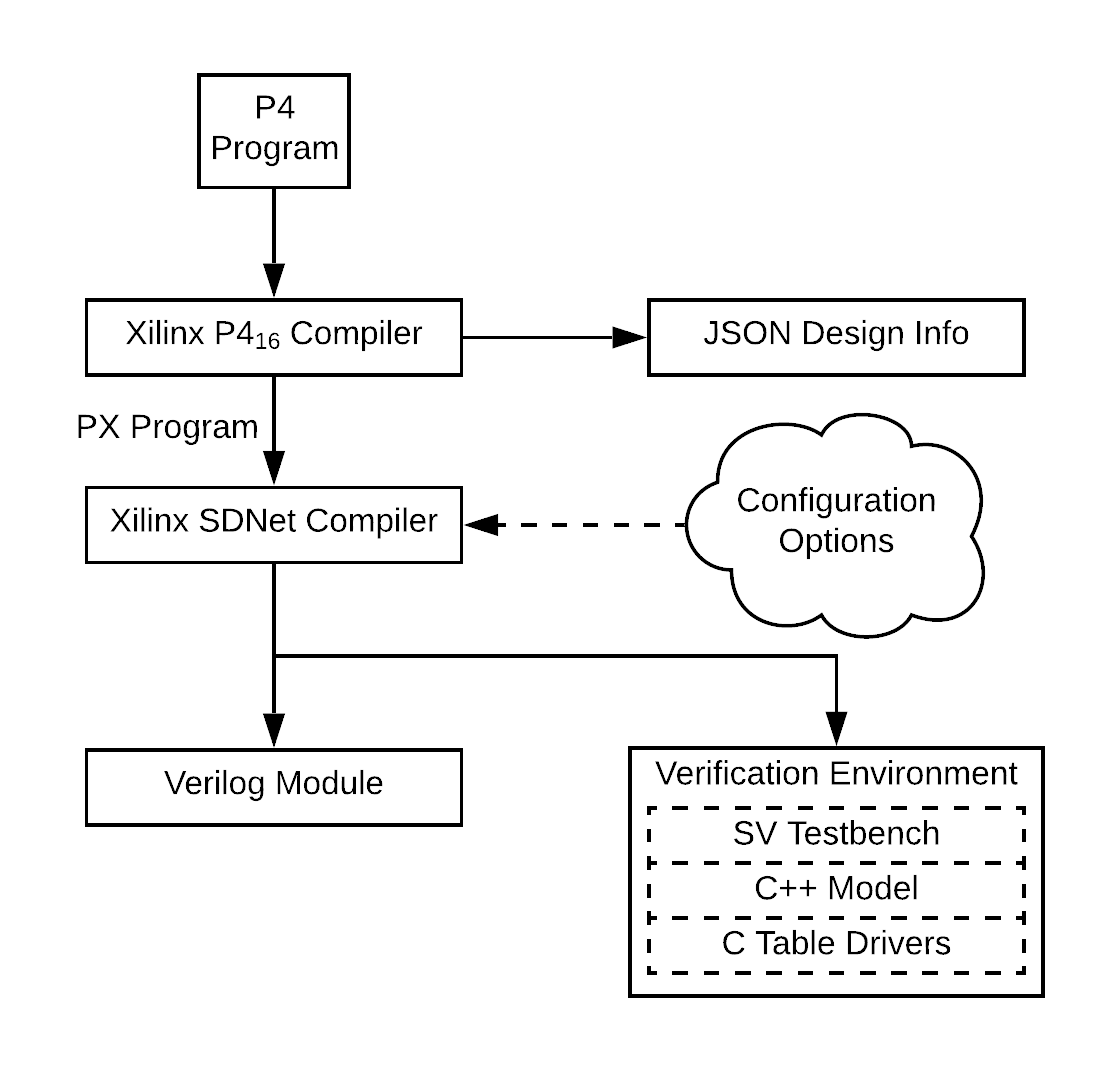
\includegraphics[width=0.7\textwidth]{sdnet.png}
	\caption{The Xilinx P4-SDNet compilation flow. P4 programs are first translated into a PX program, which is then compiled into a Verilog module using the SDNet flow. SDNet also produces a verification environment.}
	\label{sdnet}
\end{figure}

\subsection{The NetFPGA Platform}

The NetFPGA (Networked FPGA) project is a teaching and research tool designed to allow packets to be processed at line-rate in programmable hard-ware. It consists of four components: boards, tools and reference designs, a community of developers and contributed projects. The SUME board that was used in this project is the latest product in the NetFPGA hardware family. 

Figure \ref{ref-switch} depicts a block diagram of the canonical NetFPGA reference design which is used for switches, NICs, and IPv4 routers. It consists of four 10G SFP+ input/output ports along with one DMA interface for the CPU path. The NetFPGA data path consists of three main components: Input Arbiter, Output Port Lookup, and Output Queues. The Input Arbiter admits packets from the ports into the data path, towards the Output Port Lookup Module, where the main packet processing occurs and an output port is selected. The Output Queues buffer packets while they wait to be sent to the outputs. The core data path uses a 256-bit wide bus and runs sufficiently fast at 200 MHz to support an aggregate of 40 Gb/s from all four SFP+ ports.

The limitation of this platform is that it requires a substantial knowledge in both hardware design and networking, with programs written in Verilog or VHDL. To overcome this, the P4$\rightarrow$NetFPGA workflow was created to make it much easier to process packets in hardware and prototype new systems without being bogged down in hardware development.

\begin{figure}[!ht]
	\centering
	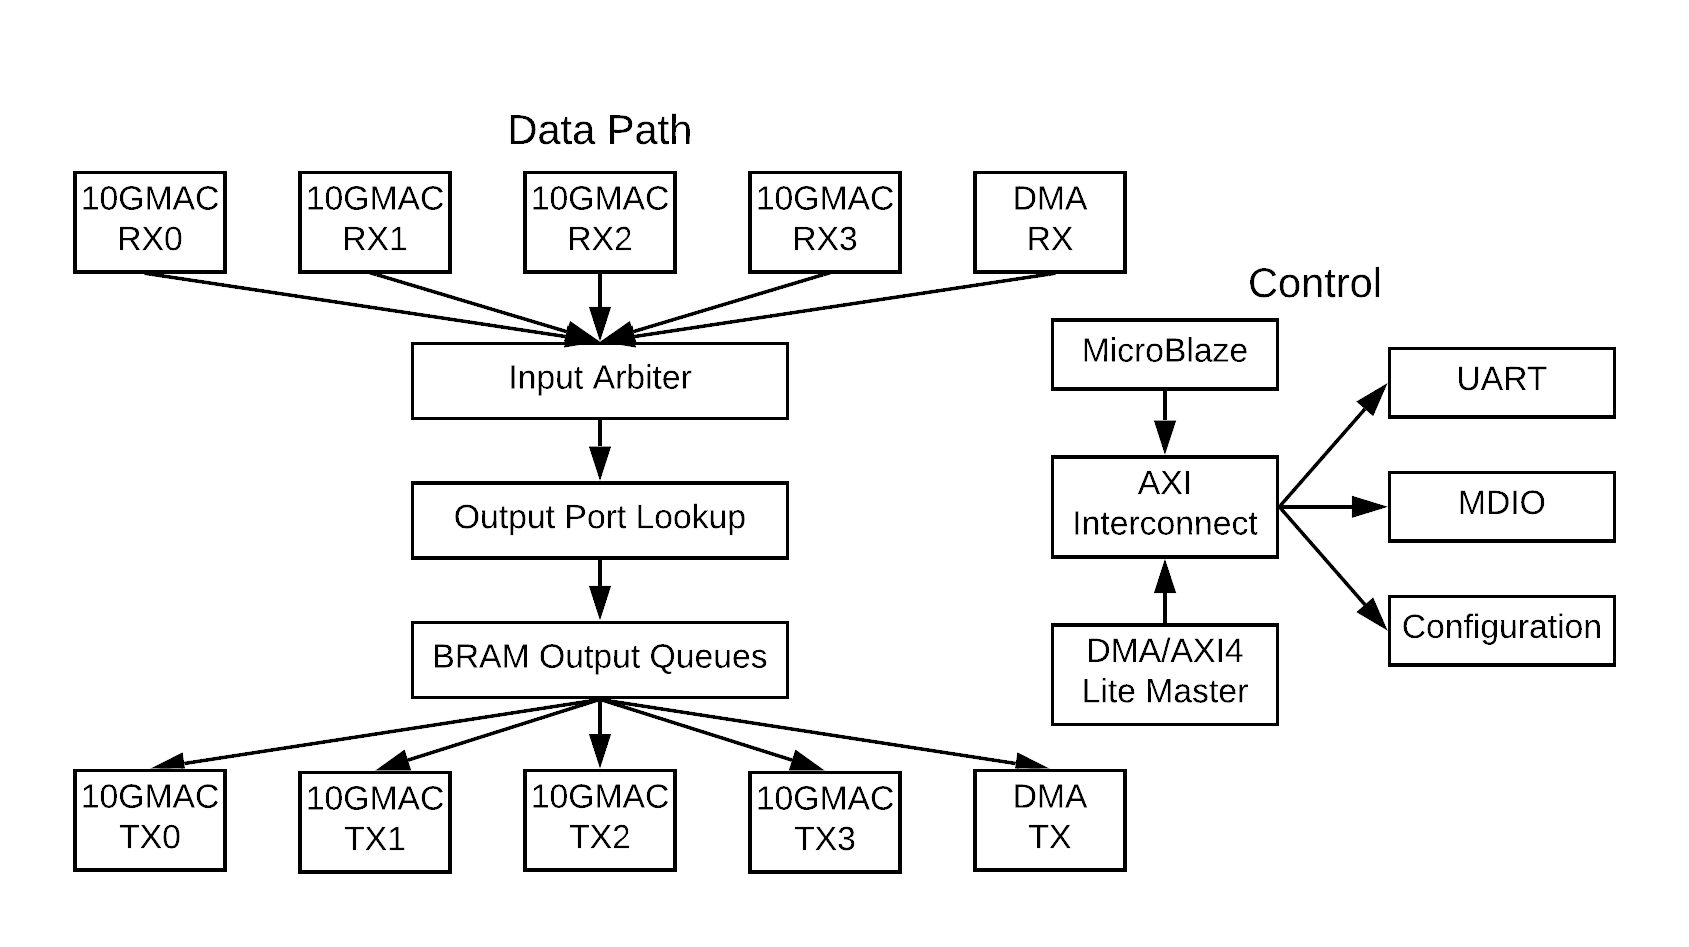
\includegraphics[width=\textwidth]{ref-switch.png}
	\caption{A block diagram of the NetFPGA reference design.}
	\label{ref-switch}
\end{figure}

\subsection{The P4$\rightarrow$NetFPGA Workflow}
The \textit{SimpleSumeSwitch} (SSS) is the P4 architecture that is currently defined for the NetFPGA SUME board. The architecture consists of a single parser, single match-action pipeline, and single deparser, as shown in Figure \ref{sss}.


%\begin{figure}
%	\centering
%	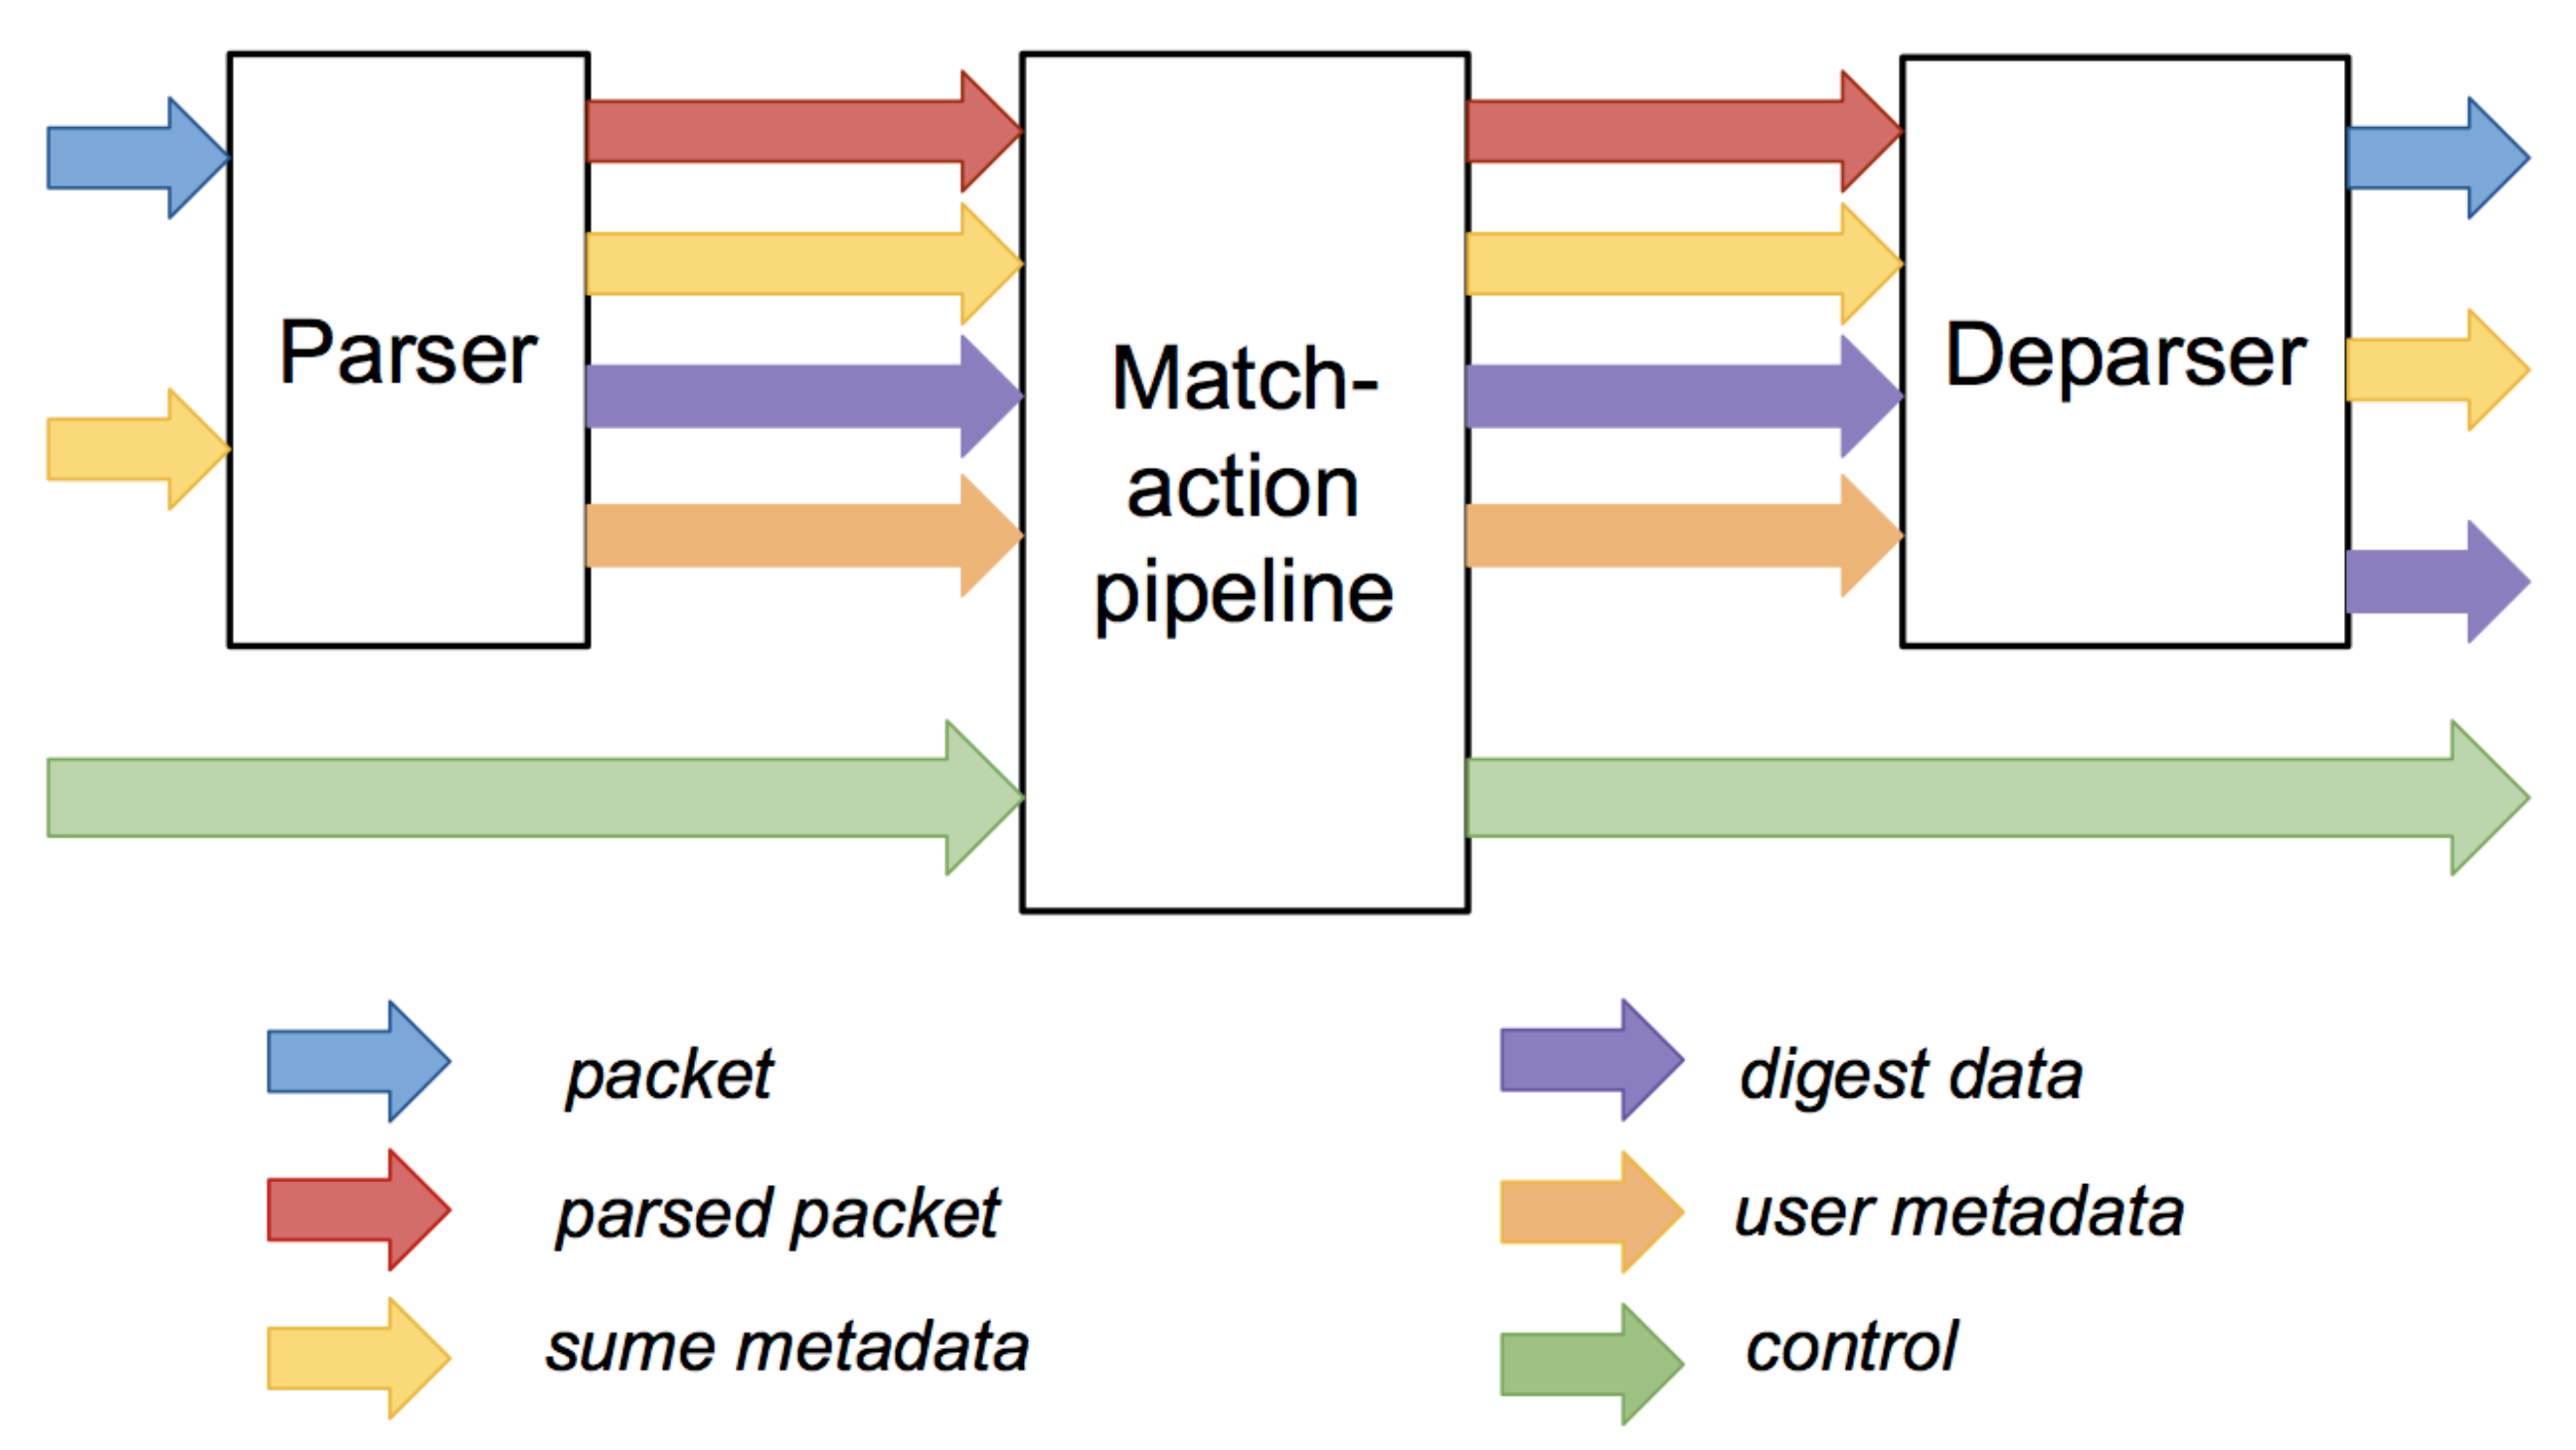
\includegraphics[width=0.8\textwidth]{sss.png}
%	\caption{The block diagram of the SimpleSumeSwitch P4 architecture used within the P4→NetFPGA workflow. Source:  
%	\label{sss}
%\end{figure}



\begin{figure}
	\centering
	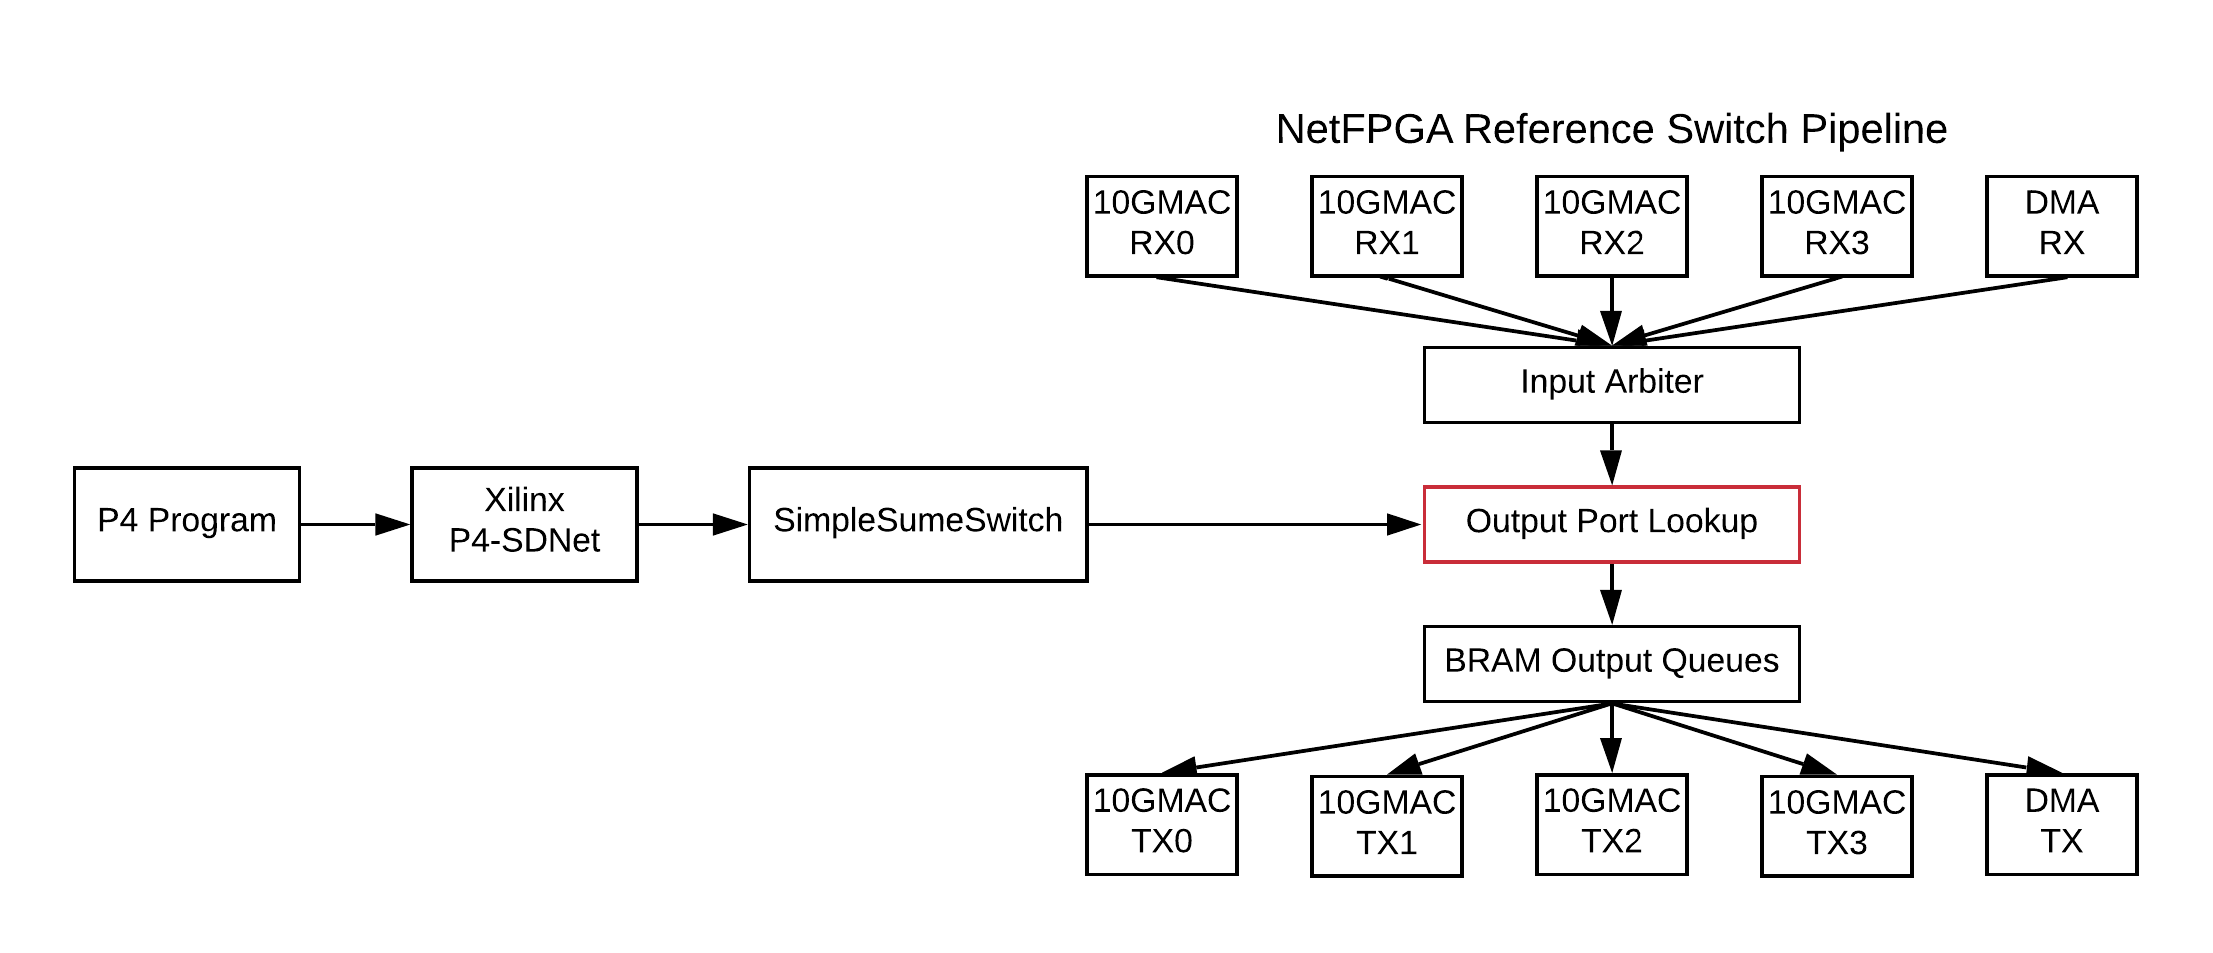
\includegraphics[width=\textwidth]{p4-netfpga.png}
	\caption{The automated P4$\rightarrow$NetFPGA compilation flow. P4 programs are compiled into an HDL instance of the SimpleSumeSwitch architecture, which is then used to replace the Output Port Lookup module in the NetFPGA Reference Switch Design.}
	\label{p4-netfpga}
\end{figure}



\subsection{High-Level Architecture}
	\subsubsection{Network Level}

	\subsubsection{System Level}
The
\subsection{Project Workflow}
	\begin{figure}
		\centering
		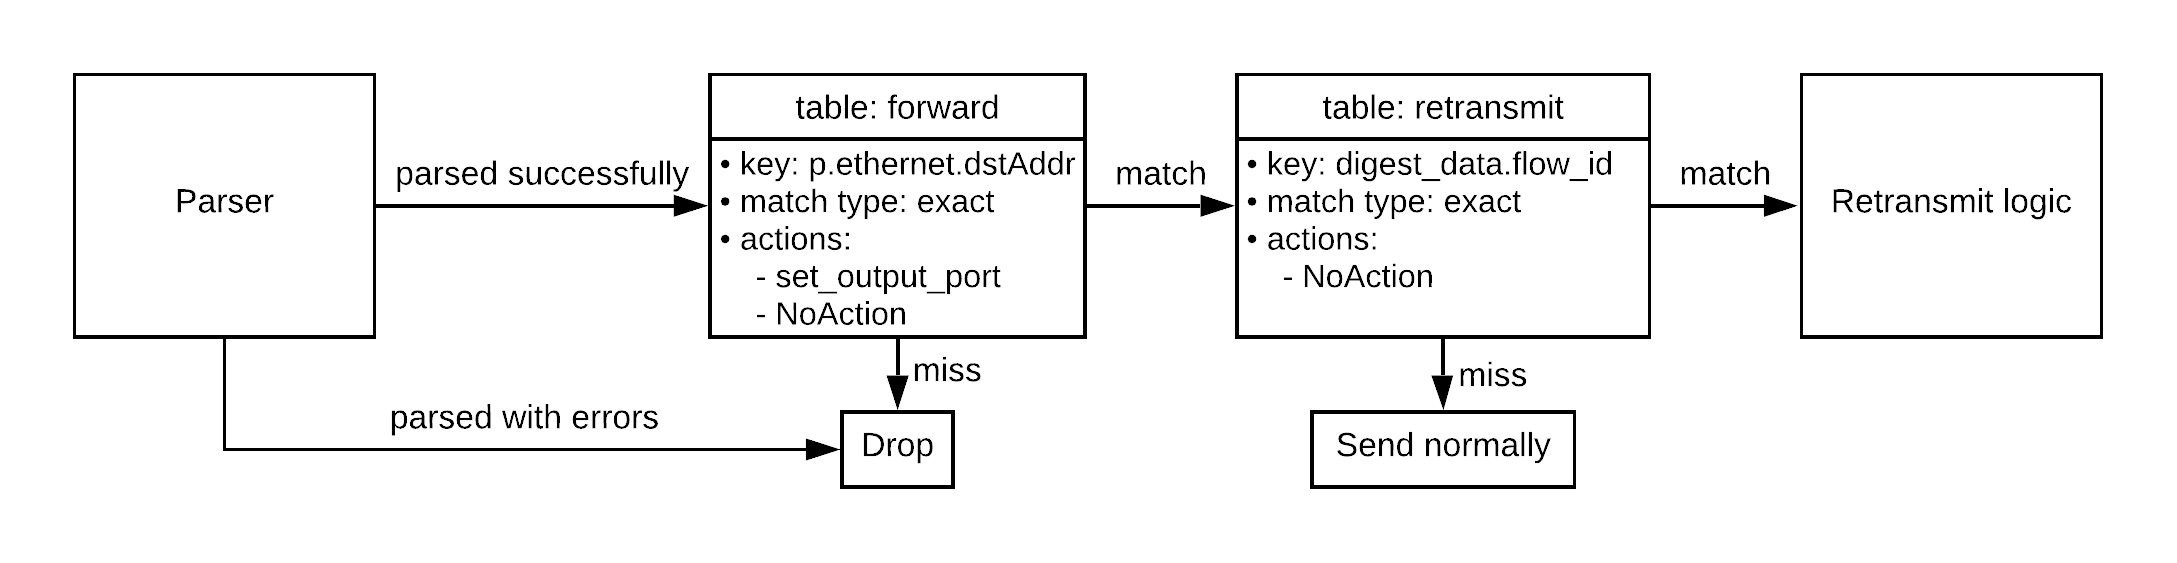
\includegraphics[width=\textwidth]{mapipe.png}
		\caption{Test}
		\label{workflow}
	\end{figure}

Figure \ref{workflow} shows the workflow for this project, according to the requirement analysis.

I will follow the \textit{spiral development model} \cite{spiral} with an iteration count equal to the number of major functionalities to add. This allows for continual implementation, testing and integration of the different functionalities.

\subsection{Risk Analysis}
The P4$\rightarrow$NetFPGA workflow is a complex platform that required the knowledge of a multitude of languages, with limited documentation \cite{fpga} and community support \cite{support}. A potential risk for the project was the difficulty of being sufficiently proficient with the platform to modify its core components and hence the inability to implement the design. Complete failure to do so was unlikely, but it could have consumed a significant amount of development time. As suggested by the spiral development model \cite{spiral}, this high-risk part was scheduled early and some “catch-up” time was allocated in the project timetable in case it caused significant delays.

\subsection{Backup Plan}	
Throughout the project development, I made sure to follow good backup procedure by keeping local weekly backups of my project using Time Machine for macOS. This provides recent history through incremental backups. I ensured additional remote storage by backing up with Microsoft OneDrive and Git, which also provided version control.